\documentclass[10pt]{article}
\usepackage[T1]{fontenc}
\usepackage{lmodern}
\usepackage[letterpaper,margin=1in]{geometry}
\usepackage{microtype}
\usepackage{amsmath,amssymb}
\usepackage{graphicx}
\usepackage{booktabs}
\usepackage{array}
\usepackage{caption}
\usepackage{enumitem}
\usepackage{xcolor}
\usepackage{tikz}
\usetikzlibrary{arrows.meta,decorations.pathreplacing}
\usepackage[numbers,sort&compress]{natbib}
\usepackage{url}
\usepackage[hidelinks]{hyperref}
\hypersetup{pdftitle={TidalMoE: Hot/Cold Expert Tiering and Host-Aware MoE Kernels for DeepSeek-V4.1-Flash on a Single NVIDIA GB300},pdfauthor={Yi-Hsiang Chen}}

% URLs may break after any of these characters (long links in the bibliography)
\makeatletter
\g@addto@macro{\UrlBreaks}{\do\/\do-\do\_\do.\do=\do?\do&}
\makeatother

\definecolor{tmblue}{HTML}{2A78D6}
\definecolor{tmorange}{HTML}{EB6834}
\definecolor{tmink}{HTML}{52514E}
\definecolor{tmhot}{HTML}{CDE2FB}
\definecolor{tmcold}{HTML}{FBE0D4}

\captionsetup{font=small,labelfont=bf}
\setlist{itemsep=1pt,topsep=3pt}
\newcolumntype{L}[1]{>{\raggedright\arraybackslash}p{#1}}
\renewcommand{\topfraction}{0.9}
\renewcommand{\bottomfraction}{0.6}
\renewcommand{\textfraction}{0.1}
\renewcommand{\floatpagefraction}{0.8}
\setlength{\bibsep}{3pt}
\setlength{\emergencystretch}{2em}
\newcommand{\figref}[1]{Figure~\ref{#1}}
\newcommand{\tabref}[1]{Table~\ref{#1}}
\newcommand{\secref}[1]{Section~\ref{#1}}

\title{{\LARGE\textbf{TidalMoE}}\\[6pt]
{\Large Hot/Cold Expert Tiering and Host-Aware MoE Kernels for Serving\\
DeepSeek-V4.1-Flash on a Single NVIDIA GB300}\\[6pt]
\large Technical Report}
\author{Yi-Hsiang Chen}
\date{November 2026}

\begin{document}
\maketitle

\begin{abstract}
DeepSeek-V4.1-Flash is a 552B-parameter mixture-of-experts (MoE) model with 196B additional Engram parameters and a
1M-token context. Its routed experts alone (${\approx}\,253$\,GiB in MXFP4) exceed the HBM of a GB300 Grace Blackwell
Ultra desktop superchip, so a single-GPU deployment must keep part of the experts in the Grace CPU's LPDDR5X and read
them over NVLink-C2C. Stock vLLM offloads whole MoE layers. Measured with the Grace uncore performance counters, that
layout is bound by host-memory reads: at 32 concurrent requests the GPU reads host memory at 258\,GB/s while HBM is
15\% active.

We present \emph{TidalMoE}, a vLLM plugin and launch configuration that requires no change to vLLM itself. It combines:
\begin{enumerate}[label=(\roman*)]
  \item per-expert hot/cold placement backed by CUDA virtual memory;
  \item an adaptive expert cache that swaps experts between tiers online and stays safe under CUDA graphs;
  \item a slot layout and per-layer host budgets fitted to how the MoE kernel schedules its work;
  \item host-aware persistent MoE kernels that read host-resident and HBM-resident experts concurrently from disjoint
        SMs inside one launch;
  \item DSpark adaptive speculative verification with a cost model measured on this machine.
\end{enumerate}
On the same hardware, model and container image, TidalMoE raises output throughput from 124 / 282 / 432 to
293 / 982 / 1862 tokens/s at 1 / 8 / 32 concurrent requests (2.4--4.3$\times$). Prefill logprobs stay bit-identical to
the unmodified model, and the 1M-token context is preserved.
\end{abstract}

\section{Introduction}
Single-node deployment of frontier MoE models is increasingly limited by memory capacity rather than compute. The
NVIDIA GB300 desktop superchip pairs a B300 GPU (HBM3e, ${\approx}\,249.5$\,GiB usable) with a 72-core Grace CPU and
${\approx}\,496$\,GB of LPDDR5X over a cache-coherent NVLink-C2C link; NVIDIA's DGX Station development
guide~\cite{dgxstationguide} documents the coherence model and notes that the GPU does not cache CPU memory. This makes
a model larger than HBM servable, provided the part that lives in host memory is chosen and accessed well.

DeepSeek-V4.1-Flash~\cite{deepseekv41} is a demanding instance of this problem.
\begin{itemize}
  \item \textbf{Structure.} 40 layers, organized as a 20-layer causal encoder followed by a 20-layer decoder whose
        global KV is projected from the encoder output. DeepSeek describes this CED design as inspired by the
        decoder--decoder architecture of YOCO~\cite{yoco}.
  \item \textbf{MoE.} Every layer contains a DeepSeekMoE block~\cite{deepseekmoe}: 1 shared expert and 384
        fine-grained routed experts, with top-6 routing.
  \item \textbf{Other components.} Engram~\cite{engram} adds 196B parameters of hashed $n$-gram ``conditional memory''
        that are looked up rather than computed. Manifold-constrained hyper-connections (mHC)~\cite{mhc} keep several
        mixed residual streams between blocks, and DSpark~\cite{dspark} provides semi-autoregressive speculative decoding with
        confidence-scheduled verification.
  \item \textbf{Size.} Experts are stored in the OCP MXFP4 microscaling format~\cite{microscaling}: 4-bit elements
        sharing a power-of-two scale per 32 values. Each routed expert takes 16.9\,MiB, so the $40 \times 384$ routed
        experts need about 253\,GiB, more than the whole HBM.
\end{itemize}
vLLM~\cite{vllm} serves the model on one GPU by offloading the experts of the first MoE layers to host memory (``UVA
offload''). It runs the TRT-LLM MoE kernels distributed with the FlashInfer kernel library~\cite{flashinfer}.

Prior MoE offloading systems, reviewed in \secref{sec:related}, almost all assume a PCIe-attached GPU on which an
expert must be copied into GPU memory before use. MoE-Infinity's trace-driven expert cache~\cite{moeinfinity} and
Pre-gated MoE's early expert selection~\cite{pregated} are typical: both exist to hide the cost of that copy.

GB300 changes the design space in three ways:
\begin{itemize}
  \item The GPU can read pinned host memory \emph{in place}, at close to the LPDDR5X bandwidth.
  \item The GPU does not cache host data across kernels.
  \item Host reads and HBM reads can proceed concurrently on disjoint SMs at their full individual rates
        (\secref{sec:char}).
\end{itemize}
Prefetching therefore adds no bandwidth on this machine. What matters is (a) how many bytes a decode step must read from
host memory, and (b) whether those reads overlap with HBM work inside the MoE kernel.

\paragraph{Contributions.}
\begin{itemize}
  \item A measurement-driven characterization of GB300 for MoE inference (\secref{sec:char}).
  \item Per-expert hot/cold placement through CUDA virtual memory, with routing-invariant expert permutation
        (\secref{sec:placement}).
  \item An adaptive expert cache with statistically gated, CUDA-graph-safe in-place swaps (\secref{sec:adapt}).
  \item A kernel-aware cold-slot layout and convex per-layer host budgets (\secref{sec:layout}).
  \item Bit-exact forced kernel tactics (\secref{sec:tactics}).
  \item Host-aware persistent MoE GEMMs that dedicate a few CTAs to host-resident experts (\secref{sec:persist}).
  \item A machine-calibrated cost model for DSpark adaptive verification (\secref{sec:av}).
  \item An end-to-end evaluation with interleaved A/B benchmarks, correctness checks and stability tests
        (\secref{sec:eval}).
\end{itemize}
The code, launch scripts, benchmark harness and raw engineering notes are in the accompanying repository.

\section{Platform and Workload Characterization}\label{sec:char}

\subsection{Hardware}
\tabref{tab:hw} summarizes the platform. Unless stated otherwise, the numbers come from microbenchmarks we ran on the
test machine: a Supermicro Super AI Station GB300 with driver 595.99 and a 64\,KiB-page Linux kernel.

How we measured:
\begin{itemize}
  \item \textbf{Reference values.} NVIDIA's Grace performance tuning guide~\cite{gracetuning} gives the platform's
        reference bandwidths.
  \item \textbf{Host traffic.} GPU-side C2C and PCIe counters (DCGM, GPM) read zero with this driver, so we used the
        Grace uncore PMUs documented in the Linux kernel~\cite{gracepmu}. The \texttt{nvidia\_nvlink\_c2c} event
        \texttt{rd\_bytes\_loc} counts GPU reads of LPDDR5X.
  \item \textbf{Host-memory allocation.} Host-resident experts are allocated with CUDA virtual memory management
        (\texttt{cuMemCreate} with a \texttt{HOST\_NUMA} location, the mechanism behind ``extended GPU memory'' in the
        CUDA programming guide~\cite{cudaegm}).
\end{itemize}

\begin{table}[!htb]
\centering\small
\caption{GB300 characteristics relevant to MoE serving (measured unless marked spec).}\label{tab:hw}
\begin{tabular}{@{}L{0.30\linewidth}L{0.66\linewidth}@{}}
\toprule
Component & Value \\
\midrule
B300 GPU & 152 SMs @ 2.07\,GHz; L2 115.5\,MiB; HBM3e 7.16\,TB/s spec, 6.4--6.6\,TB/s streaming read \\
Grace CPU & 72 Neoverse V2 cores; LPDDR5X 396\,GB/s spec (360\,GB/s per firmware) \\
NVLink-C2C & $10 \times 44.7 = 447$\,GB/s per direction, cache-coherent \\
GPU read of pinned host memory & 383--390\,GB/s with \texttt{cuMemCreate} (\texttt{HOST\_NUMA}); 346--353\,GB/s with \texttt{malloc} or \texttt{cudaHostAlloc} \\
Per-SM read limit & 51.2\,GB/s through TMA with ${\geq}\,4$ stages in flight, for HBM and host memory alike \\
Read latency (pointer chase) & HBM 134--145\,ns; pinned host memory 634--704\,ns \\
L2 caching of host data & None: re-reading 64\,MB of host data stays at 383\,GB/s \\
Concurrent host + HBM reads & Host 389\,GB/s on 16 SMs \emph{and} HBM 6.62\,TB/s on the other 136 SMs, at the same time \\
Copy engine, host to HBM & 188 / 253 / 303 / 365 / ${\approx}\,389$\,GB/s for 1 / 2 / 4 / 16 / ${\geq}\,64$\,MB chunks \\
CPU memory traffic & Halves GPU host-read bandwidth (386 to 189\,GB/s) \\
\bottomrule
\end{tabular}
\end{table}

\begin{figure}[!t]
\centering
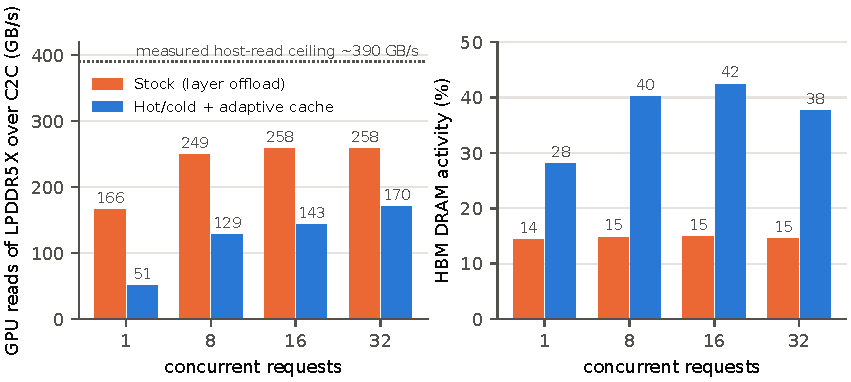
\includegraphics[width=\linewidth]{figures/fig_bandwidth.pdf}
\caption{Memory traffic under steady ShareGPT load. Left: GPU reads of LPDDR5X over NVLink-C2C, measured with the Grace
uncore PMU. Right: HBM DRAM activity, from the GPM counter. Stock layer offload saturates at 258\,GB/s of host reads
with HBM nearly idle. Per-expert hot/cold placement with the adaptive cache cuts host traffic per step by 3.8$\times$
and raises HBM activity 2--3$\times$.}\label{fig:bw}
\end{figure}

\paragraph{Three facts shape the design.}
\begin{itemize}
  \item \textbf{The limit is LPDDR5X, not the link.} With enough bytes in flight the GPU reads host memory at 98\% of
        the LPDDR5X specification. Reaching that takes only 8--16 SMs with deep TMA pipelines.
  \item \textbf{Host and HBM reads are additive.} The two run at full rate concurrently, but only if different SMs
        issue them.
  \item \textbf{Copy engines are not an alternative.} They are slow for expert-sized (1--4\,MB) chunks and share the
        same LPDDR5X bandwidth.
\end{itemize}
Fiddler~\cite{fiddler} executes experts whose weights sit in host memory on the CPU instead of transferring them. This
does not pay off here: the Grace CPU needs 0.80\,ms for 11 experts, the GPU reads the same experts in 0.61\,ms, and the
CPU's own memory traffic slows the GPU's host reads.

\subsection{Why stock offloading is host-bound}
\figref{fig:bw} (orange) shows the stock layout under load. Experts of layers 0--8 live in host memory, so ${\approx}\,24\%$
of each token's expert reads cross C2C. From 16 concurrent requests on, GPU reads of host memory plateau at 258\,GB/s.
The SMs are 91--93\% active, mostly stalled on those reads, while HBM activity stays at ${\approx}\,15\%$.

Nsight Systems and Nsight Compute traces of the TRT-LLM MoE GEMMs explain why the plateau sits below the 390\,GB/s
ceiling:
\begin{itemize}
  \item The kernel launches CTAs in (tile, expert) order.
  \item The 36--40 CTAs of a host-resident expert each hold an SM for a long time.
  \item Once host bandwidth saturates, cold CTAs occupy every SM and HBM work stalls behind them.
\end{itemize}
Host and HBM reads therefore \emph{serialize} instead of overlapping.


\subsection{Routing skew}
We captured per-token routing for all 40 layers with vLLM's \texttt{--enable-return-routed-experts}. The traffic
covered three workloads: English chat (ShareGPT~\cite{sharegpt}), Chinese chat (ShareGPT-CN~\cite{sharegptcn}) and
code.

\figref{fig:skew} shows strong skew. The most-used 20\% of each layer's experts receive 61--74\% of decode routing; the
least-used 24\% receive only 0.7--2.7\%.

The hot sets, however, are domain-specific. The average Jaccard similarity of per-layer top-20\% sets is 0.34 between
English and Chinese, 0.38 between English and code, and 0.20 between Chinese and code. Other studies report the same:
\begin{itemize}
  \item Patterns behind Chaos~\cite{patternschaos} profiled expert data movement of four 200B--1000B MoE models over
        more than 24,000 requests and found structured temporal and spatial patterns.
  \item ST-MoE~\cite{stmoe} found that expert requests correlate strongly within an application domain.
  \item FineMoE~\cite{fmoe} exploits semantic hints from prompts to anticipate expert selection.
\end{itemize}
A static placement therefore helps mainly the traffic it was built from. This motivates the adaptive cache of
\secref{sec:adapt}.

\begin{figure}[!htb]
\centering
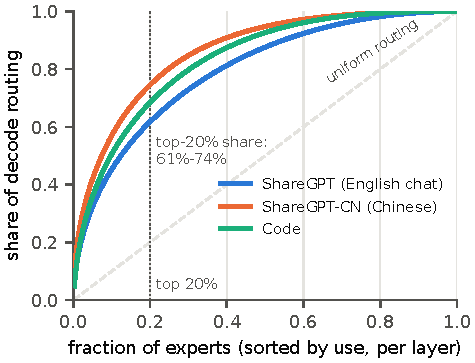
\includegraphics[width=0.55\linewidth]{figures/fig_routing_skew.pdf}
\caption{Cumulative share of decode routing versus fraction of experts, sorted by use within each layer and averaged
over the 40 layers.}\label{fig:skew}
\end{figure}

\section{Design}\label{sec:design}
TidalMoE is a vLLM \emph{general plugin}, loaded through \texttt{PYTHONPATH} and an entry point, together with a launch
script for the unmodified \texttt{vllm/vllm-openai} v0.33.0 image. Each feature sits behind its own environment
variable and can be switched off independently.

\subsection{Per-expert hot/cold placement}\label{sec:placement}
The plugin wraps the model's \texttt{process\_weights\_after\_loading}. It therefore runs after the MoE kernel has
converted the checkpoint into its own weight layout, and before vLLM profiles memory for the KV cache. For each layer it
does two things.

\textbf{Permute the experts.} The experts are reordered so that a placement plan's hot experts occupy the leading
physical slots. Every tensor with a leading expert dimension is permuted the same way: weights, block scales, clamp
limits, gate-projection rows, and the text and image routing-correction biases. Routing decisions are therefore
unchanged; only each expert's physical slot moves.

\textbf{Rebuild \texttt{w13} and \texttt{w2}.} Each tensor is rebuilt on one contiguous CUDA virtual-address range
(\texttt{cuMemAddressReserve}, \texttt{cuMemCreate}, \texttt{cuMemMap}). Each 2\,MiB page is backed by HBM when its slot
is hot, and by pinned LPDDR5X on NUMA node 0 when it is cold (\figref{fig:vmm}).

The kernel sees an ordinary CUDA tensor; host-resident slots are simply slower to read. The default plan keeps 3,312
cold experts (54.2\,GiB) in host memory and 198.95\,GiB of experts in HBM.

\begin{figure}[!htb]
\centering
\begin{tikzpicture}[x=0.42cm,y=0.55cm,font=\footnotesize]
  \foreach \i in {0,...,31} {
    \pgfmathtruncatemacro{\c}{mod(\i,5)==2 ? 1 : 0}
    \ifnum\c=1
      \fill[tmcold,draw=tmorange,line width=0.5pt] (\i,0) rectangle ++(1,1);
    \else
      \fill[tmhot,draw=tmblue,line width=0.5pt] (\i,0) rectangle ++(1,1);
    \fi
  }
  \node[anchor=east,align=right] at (-0.3,0.5) {\texttt{w13} virtual\\address range};
  \draw[decorate,decoration={brace,amplitude=4pt}] (0,1.2) -- (32,1.2)
     node[midway,above=4pt] {one layer's 384 expert slots (schematic); cold slots in groups of 8, spread evenly};
  \node[draw=tmblue,fill=tmhot,rounded corners=2pt,align=center,minimum width=4.8cm] (hbm) at (8,-2.6)
     {HBM3e pages: hot experts\\[1pt] {\color{tmink}read at up to 6.6\,TB/s}};
  \node[draw=tmorange,fill=tmcold,rounded corners=2pt,align=center,minimum width=5.6cm] (lp) at (24,-2.6)
     {pinned Grace LPDDR5X pages: cold experts\\[1pt] {\color{tmink}read in place over NVLink-C2C, ${\leq}\,390$\,GB/s}};
  \draw[-{Stealth[length=5pt]},tmblue] (5.5,-0.05) -- (hbm.north);
  \draw[-{Stealth[length=5pt]},tmorange] (17.5,-0.05) -- (lp.north west);
  \draw[-{Stealth[length=5pt]},tmorange] (27.5,-0.05) -- (lp.north);
\end{tikzpicture}
\caption{Per-expert placement. Each MoE weight tensor is a single CUDA virtual-address range whose 2\,MiB pages are
backed by HBM or by pinned host memory. Experts are permuted, together with every per-expert tensor and the routing
biases, so that the cold slots form small groups spread evenly over the layer.}\label{fig:vmm}
\end{figure}

\subsection{Adaptive expert cache}\label{sec:adapt}
A static plan is only a starting point, because hot sets drift with the domain. The adaptive cache works in three steps.
\begin{itemize}
  \item \textbf{Counting.} Inside every decode-size MoE call (${\leq}\,128$ tokens), a fused Triton kernel adds one per
        \emph{distinct} expert touched to a per-layer GPU counter; these are the reads the step actually pays for.
        Large prefill chunks are not counted, and the kernel runs inside the CUDA graphs.
  \item \textbf{Scoring.} Every 3\,s the engine thread reads the counters and updates an exponential moving average
        $s \leftarrow \beta s + c$ with $\beta = 0.5^{1/10}$, a half-life of 10 epochs.
  \item \textbf{Swapping.} The hottest host-resident expert $x$ is paired with the coldest HBM-resident expert $y$ and
        swapped only if
        \begin{equation}
          s_x > (1+m)\, s_y \quad\text{and}\quad s_x - s_y > z \sqrt{s_x + s_y + 1},\qquad m = 0.25,\ z = 3 .
        \end{equation}
        The second condition is a Poisson significance test, so sampling noise does not cause churn. At most 64 swaps
        are made per epoch, ranked by expected benefit.
\end{itemize}

A swap exchanges the two slots' \emph{rows} in every per-expert tensor, including the gate rows and routing biases. Two
properties follow:
\begin{itemize}
  \item Device addresses never change, so captured CUDA graphs stay valid.
  \item The logical model is unchanged: prefill logprobs remained bit-identical after more than 1,100 live swaps.
\end{itemize}

Related adaptive policies exist in offloading systems:
\begin{itemize}
  \item HybriMoE~\cite{hybrimoe} keeps a score-based expert cache to cope with unstable activation patterns.
  \item DALI~\cite{dali} replaces GPU cache entries using the temporal correlation of expert workloads.
  \item TriMoE~\cite{trimoe} rebalances experts across tiers with prediction-driven dynamic relayout.
  \item Prism~\cite{edgeplacement} migrates experts at runtime as workloads change.
\end{itemize}
Our cache differs in two respects. Its swaps are gated by a significance test, and it reuses fixed slots by exchanging
rows in place, which keeps CUDA graphs valid.

\figref{fig:adapt} shows the cache recovering from a mismatched plan. Chinese traffic served from a plan built without
Chinese data starts with 23.5\% of routed selections in host memory. The cache brings this below 3\% within about
6 minutes, using 5,617 swaps. On that traffic it raised throughput at 32 concurrent requests from 644 to 1,150 tokens/s.

\begin{figure}[!htb]
\centering
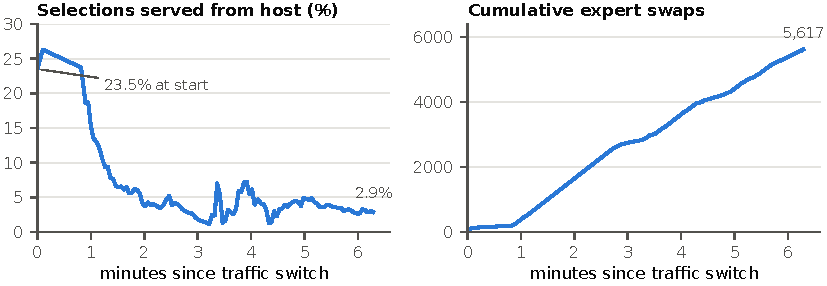
\includegraphics[width=\linewidth]{figures/fig_adapt.pdf}
\caption{Adaptive expert cache under a domain shift: Chinese traffic on a plan built without Chinese data. Left: share of
routed expert selections served from host memory, per 3\,s epoch. Right: cumulative swaps.}\label{fig:adapt}
\end{figure}

\subsection{Kernel-aware layout and per-layer budgets}\label{sec:layout}
\paragraph{Groups of 8.} The TRT-LLM kernel issues CTAs in expert-slot order, so contiguous runs of cold slots produce
bursts of host-bound CTAs that occupy many SMs at once. We therefore place cold slots in groups of 8 experts, spread
evenly across the layer. For \texttt{w13}, 8 experts fill exactly 45 pages of 2\,MiB. Each group's \texttt{w2} shares
one half page with a hot neighbour, and that page stays in HBM. This layout gave $+3$--$6\%$ at 32 concurrent requests.

\paragraph{Convex per-layer budgets.} Nsight traces show that a MoE layer costs roughly
$\max(t_\text{HBM},\, c \cdot n_\text{cold})$ per step, with $c \approx 64\,\mu$s per touched cold expert for the
TRT-LLM kernel. Cold experts are thus nearly free up to a crossover point and expensive beyond it, and the original plan
left some layers above the crossover while others had slack. A greedy allocation over this convex cost, weighted over
1, 8 and 32 concurrent requests, moves host budget from host-bound layers to layers with slack.

\subsection{Bit-exact forced kernel tactics}\label{sec:tactics}
FlashInfer's autotuner ran on synthetic, uniform routing and selected 3-stage pipelines (115--141\,KB of shared memory)
for the decode token buckets. With real, skewed routing and host-resident tiles, deeper pipelines are faster: 4--6
stages, or a 512-wide K tile (179--224\,KB), keep more bytes in flight. We force one tactic per token bucket.

Some tactics change the split-K reduction order and therefore the result. An exhaustive search over all 1,440 tactics
of the 8-token bucket found 160 that are bit-identical to the autotuned choice, and we use the fastest of these. The
forced tactics remain in use for the calls that still run on TRT-LLM: prefill chunks and the DSpark drafter.

\subsection{Reclaiming HBM for hot experts}
Every GiB of HBM holds ${\approx}\,60$ more hot experts. We reclaim HBM in two ways.

\textbf{KV sized to the context limit.} GPU KV is sized to exactly one 1M-token request (1,085,568 tokens, 2.1\,GiB)
instead of filling the GPU-utilization budget. A 32\,GiB CPU KV tier (vLLM's \texttt{SimpleCPUOffloadConnector}) serves
prefix reuse beyond that.

\textbf{Token embedding on the host.} The 1.23\,GiB token embedding is only gathered from (about 64 rows per step), so
it moves to pinned host memory.

\subsection{Host-aware persistent MoE kernels}\label{sec:persist}
The remaining loss is the serialization of host and HBM reads inside the MoE GEMMs (\secref{sec:char}). We replace the
TRT-LLM path for every routed-expert call of up to 128 tokens: decode, speculative verification and short prefill
chunks. Each such call runs four launches, chained with programmatic dependent launch and captured in CUDA graphs:
\begin{enumerate}
  \item A Triton \emph{front} kernel builds a routing record with cold tiles first and gathers MXFP8 activations.
  \item A persistent GEMM1 (gate/up projection with fused SwiGLU and clamp), with one CTA per SM and a 6-stage TMA
        pipeline.
  \item A persistent GEMM2 (down projection) with a 10-stage pipeline.
  \item A Triton finalize that computes the top-$k$ weighted sum, when vLLM does not defer it.
\end{enumerate}

In both GEMMs, CTAs $[0, k_c)$ take every cold tile first and stream it from host memory over C2C, while the other
$152 - k_c$ CTAs stream HBM (\figref{fig:cta}). The front kernel chooses $k_c \in [4, 16]$ per call from a bandwidth
model. This reproduces, inside a single launch, the concurrent host+HBM regime of \tabref{tab:hw}.

The GEMMs are generated by exact text edits from vLLM's CuTe-DSL~\cite{cutlass} routed-expert kernels. In the image
these exist only for a 4-GPU (TP4) configuration with at most 8 rows; we extend them to one GPU and up to 128 rows. As a
result they:
\begin{itemize}
  \item read precisely the TRT-LLM weight and scale layout that vLLM prepares, so no second copy of the weights is
        needed;
  \item keep the same MMA order and epilogue arithmetic, so rows are bit-identical to TRT-LLM's non-split-K tactics in
        standalone tests.
\end{itemize}

\begin{figure}[!htb]
\centering
\begin{tikzpicture}[font=\footnotesize]
  \foreach \i in {0,...,23} {
    \pgfmathtruncatemacro{\h}{\i<3 ? 1 : 0}
    \ifnum\h=1
      \fill[tmcold,draw=tmorange,line width=0.5pt] (\i*0.55,0) rectangle ++(0.46,1);
    \else
      \fill[tmhot,draw=tmblue,line width=0.5pt] (\i*0.55,0) rectangle ++(0.46,1);
    \fi
  }
  \node[anchor=east] at (-0.2,0.5) {CTAs (one per SM)};
  \draw[decorate,decoration={brace,amplitude=4pt,mirror}] (0,-0.1) -- (1.56,-0.1)
     node[midway,below=5pt,align=center] {$k_c$ CTAs (4--16 of 152):\\cold tiles, deep TMA};
  \draw[decorate,decoration={brace,amplitude=4pt,mirror}] (1.65,-0.1) -- (13.11,-0.1)
     node[midway,below=5pt] {remaining CTAs: hot tiles from HBM, in routing-record order};
  \node[draw=tmorange,fill=tmcold,rounded corners=2pt,align=center] (lp) at (0.78,2.4) {LPDDR5X\\${\sim}\,380$\,GB/s};
  \node[draw=tmblue,fill=tmhot,rounded corners=2pt,align=center] (hb) at (7.4,2.4) {HBM3e\\${\sim}\,6$\,TB/s};
  \draw[-{Stealth[length=5pt]},tmorange] (lp.south) -- (0.78,1.05);
  \draw[-{Stealth[length=5pt]},tmblue] (hb.south) -- (7.4,1.05);
\end{tikzpicture}
\caption{Work split in the host-aware persistent GEMMs. Within one launch per GEMM, a few CTAs own all host-resident
(cold) tiles and keep enough bytes in flight to saturate LPDDR5X, while the rest stream HBM without waiting behind
host reads.}\label{fig:cta}
\end{figure}

\begin{table}[!htb]
\centering\small
\caption{One MoE layer at 64 tokens with 12 host-resident experts touched (Nsight Compute, standalone, production
layout).}\label{tab:ncu}
\begin{tabular}{@{}lrrrr@{}}
\toprule
Kernel & GEMM1 time & host read & HBM read & GEMM2 time \\
\midrule
TRT-LLM (production path) & 534\,$\mu$s & 265\,GB/s & 4.10\,TB/s & 252\,$\mu$s \\
TidalMoE persistent & 375\,$\mu$s & 378\,GB/s & 5.97\,TB/s & 187\,$\mu$s \\
\bottomrule
\end{tabular}
\end{table}

\paragraph{Measured effect.} \tabref{tab:ncu} and \figref{fig:persist} show the result.
\begin{itemize}
  \item \textbf{Both tiers at once.} The persistent kernels reach 378\,GB/s of host reads, near the 390\,GB/s ceiling,
        \emph{concurrently} with 5.97\,TB/s of HBM reads.
  \item \textbf{Layer time.} A whole MoE layer takes 24--30\% less time with 4--18 cold experts.
  \item \textbf{Few cold experts.} Both kernels are HBM-bound at ${\approx}\,6$\,TB/s and perform alike. The one
        exception is 32 tokens with 0--2 cold experts, where the persistent path is 2--4\% slower because of its front
        kernel.
  \item \textbf{Many cold experts.} Beyond about 11 cold experts per layer at 64 tokens, each additional cold expert
        costs ${\approx}\,46\,\mu$s, which is its 17.7\,MB at ${\approx}\,380$\,GB/s. There the kernel is at the
        hardware limit.
\end{itemize}

\begin{figure}[!htb]
\centering
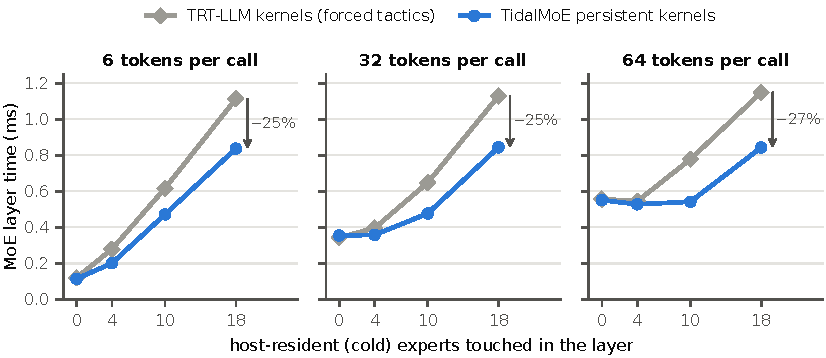
\includegraphics[width=\linewidth]{figures/fig_persist.pdf}
\caption{Time of one MoE layer versus the number of host-resident experts touched, at 6, 32 and 64 tokens per call.
Standalone benchmark with realistic routing and the production host/HBM layout.}\label{fig:persist}
\end{figure}

\subsection{DSpark adaptive verification with a measured cost model}\label{sec:av}
DSpark~\cite{dspark} drafts up to 5 tokens per request, and a confidence head predicts each draft's acceptance
probability. vLLM's adaptive verification ranks all (request, position) drafts by survival probability. It then
verifies the budget $n$ that maximizes expected accepted tokens per unit time. The time of a step with $r$ running
requests and $n$ target tokens is modelled as $t_\text{draft}(r) + t_\text{verify}(n)$. With rejection sampling,
speculative decoding preserves the target model's output distribution~\cite{specdec}, so this is purely a performance
decision.

\textbf{The problem.} vLLM measures $t_\text{verify}$ at startup with padding tokens that route to no expert, so the
profile omits the MoE cost. On GB300 that cost is large: every extra verified token can pull in more host-resident
experts. With the built-in curve, adaptive verification \emph{lost} 4--9\% at 1, 8 and 32 concurrent requests.

\textbf{The fix.} We replace both terms with values measured on the machine with the persistent kernels:
$t_\text{draft}(r) \approx 0.1\,r$\,ms, and $t_\text{verify}(n)$ taken from the pure-decode step time per CUDA-graph
size, from 7.3\,ms at 1 token to 39\,ms at 128 tokens. Pruning is enabled only when at least 2 requests are running,
because at 1 request it cost 3\%.

\textbf{The result} is shown in \figref{fig:av}. Throughput rises by up to 14\% at 32 concurrent requests, where the
acceptance length goes from 1.77 to 2.49 and median TPOT from 18.9 to 15.5\,ms. No concurrency level regresses.

\begin{figure}[!htb]
\centering
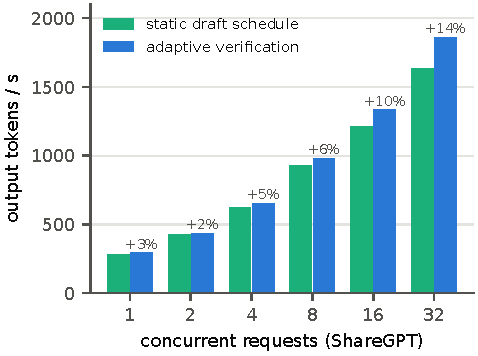
\includegraphics[width=0.55\linewidth]{figures/fig_av.pdf}
\caption{DSpark adaptive verification with the machine-calibrated cost model, compared with the static draft schedule.
Each bar is the mean of 2 interleaved runs.}\label{fig:av}
\end{figure}

\section{Evaluation}\label{sec:eval}

\paragraph{Setup.}
\begin{itemize}
  \item \textbf{Software.} The \texttt{vllm/vllm-openai} v0.33.0 image (FlashInfer 0.7.2.post1, PyTorch 2.14, CUDA
        13.0) with DeepSeek-V4.1-Flash-1017: MXFP4 experts, Engram in pinned host memory, DSpark speculative decoding.
  \item \textbf{Stock baseline.} The same image and model with vLLM's layer-wise UVA expert offload, the default DSpark
        schedule, and up to 24 concurrent sequences.
  \item \textbf{Load generator.} vllm-bench~\cite{vllmbench}, a Rust benchmark client for vLLM endpoints, driving the
        chat API.
  \item \textbf{Prompts.} ShareGPT~\cite{sharegpt}, or 4,000 first-turn Chinese prompts from ShareGPT-CN~\cite{sharegptcn}.
  \item \textbf{Requests.} 1,024 output tokens with EOS ignored, temperature 0, and 4 prompts per unit of concurrency at
        each point.
  \item \textbf{Procedure.} Every run starts a fresh server and warms up with 96 prompts at 16 concurrent requests before
        benchmarking.
\end{itemize}
Run-to-run noise is about $\pm 2.5\%$ at 8 and 32 concurrent requests. Every improvement was therefore measured against
its predecessor in the same session, with configurations interleaved (A B B A) and at least two runs each.

\begin{figure}[!t]
\centering
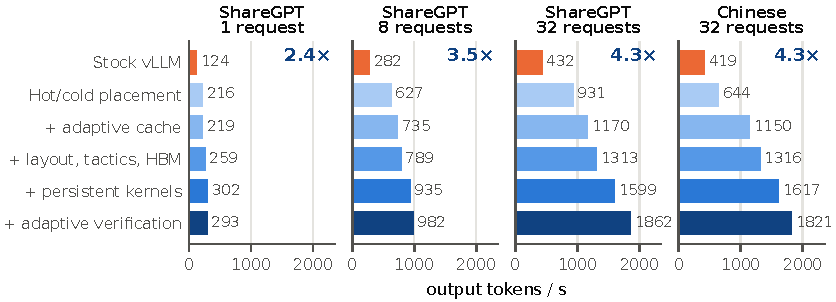
\includegraphics[width=\linewidth]{figures/fig_progression.pdf}
\caption{Output throughput after each optimization stage. Each stage was verified against the previous one in
interleaved A/B runs. The Chinese bar of the first placement stage uses a plan built without Chinese data.}\label{fig:prog}
\end{figure}

\subsection{Throughput}
\figref{fig:prog} shows the cumulative effect of each stage, and \figref{fig:conc} and \tabref{tab:final} show full
concurrency sweeps. The final configuration delivers 2.4$\times$ at 1, 3.5$\times$ at 8 and 4.3$\times$ at
32 concurrent requests over stock vLLM. The largest single steps are placement plus the adaptive cache at medium and
high concurrency, the persistent kernels at every concurrency (+16--24\%), and calibrated adaptive verification at high
concurrency (+12--14\%).

\begin{figure}[!htb]
\centering
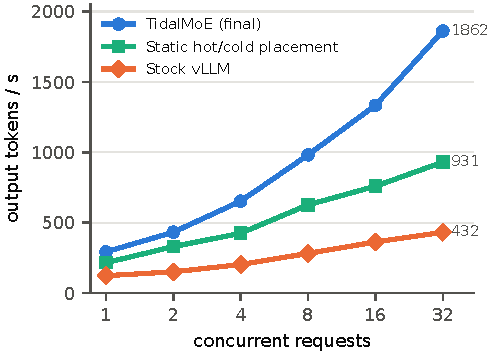
\includegraphics[width=0.55\linewidth]{figures/fig_concurrency.pdf}
\caption{Output throughput versus concurrency (ShareGPT, 1024 output tokens) for stock vLLM, the first static placement
and the final TidalMoE configuration.}\label{fig:conc}
\end{figure}

\begin{table}[!htb]
\centering\small
\caption{Final throughput (output tokens/s; means of interleaved runs) versus stock vLLM on the same machine.}\label{tab:final}
\begin{tabular}{@{}lrrrrrrr@{}}
\toprule
& \multicolumn{6}{c}{ShareGPT, concurrent requests} & Chinese \\
\cmidrule(lr){2-7}
& 1 & 2 & 4 & 8 & 16 & 32 & 32 \\
\midrule
Stock vLLM & 124 & 151 & 203 & 282 & 364 & 432 & 419 \\
TidalMoE & 293 & 433 & 653 & 982 & 1334 & 1862 & 1821 \\
Speed-up & 2.4$\times$ & 2.9$\times$ & 3.2$\times$ & 3.5$\times$ & 3.7$\times$ & 4.3$\times$ & 4.3$\times$ \\
\bottomrule
\end{tabular}
\end{table}

\begin{table}[!t]
\centering\small
\caption{Alternatives that were implemented or measured and rejected (or kept for another reason).}\label{tab:rejected}
\begin{tabular}{@{}L{0.36\linewidth}L{0.60\linewidth}@{}}
\toprule
Alternative & Outcome \\
\midrule
Hot and cold experts as two concurrent TRT-LLM calls & Slower: the cold-only call reads host memory at ${\sim}\,200$\,GB/s with a shallow pipeline \\
SM partitioning with CUDA green contexts & Loses at ${\leq}\,12$ cold experts per layer; not bit-exact \\
Cold experts computed on the Grace CPU & 0.80\,ms vs.\ 0.61\,ms for the GPU to read them; CPU traffic also slows GPU host reads \\
Copy-engine prefetch of cold experts & Routing is known only at the layer; copy engines reach 188--303\,GB/s for 1--4\,MB chunks \\
DeepGEMM Mega-MoE~\cite{deepgemm} & 3--14\% slower with host-resident experts; +0.9\,GiB of buffers \\
Mega-mHC for steps of ${\leq}\,16$ tokens & No gain \\
Restoring the cache state across restarts & +2--3\% right after a restart only; most of the slump is first-request JIT \\
CPU KV tier & Throughput-neutral; kept for prefix reuse beyond the 1M-token GPU KV \\
\bottomrule
\end{tabular}
\end{table}

\subsection{Where the time goes now}
At 32 concurrent requests, the persistent kernels read host memory at 375--379\,GB/s against a ceiling of
${\approx}\,385$--$390$\,GB/s, and about 15--18 cold experts per layer are touched per step. Decode is therefore again
bound by host-memory bandwidth, but now at the hardware limit rather than at 66\% of it. Further gains require fewer host
bytes per step rather than faster kernels: either more HBM for hot experts, or better prediction of \emph{which} experts
will be needed (\secref{sec:related}).

\subsection{Correctness}
\begin{itemize}
  \item \textbf{Bit-preserving stages.} Placement, adaptive swaps, forced tactics, the embedding move and the KV sizing
        are all bit-preserving. Teacher-forced prefill logprobs on three reference texts (English, Chinese and code;
        352 tokens) match the unmodified model exactly.
  \item \textbf{Persistent kernels.}
        \begin{itemize}
          \item At ${\leq}\,8$ tokens they replace a split-K reduction with a non-split-K one. Decode is therefore
                deterministic but not bit-identical to TRT-LLM, and greedy outputs change at near-ties.
          \item Quality is unchanged. Over 13.3k greedy tokens re-scored teacher-forced, 2.93\% are not the argmax,
                versus 3.01\% for TRT-LLM, and the mean $|\Delta\log p|$ is 0.048 for both.
          \item Long generations of up to 2,048 tokens in English, Chinese, code and math stay coherent and correct.
        \end{itemize}
  \item \textbf{Adaptive verification.} It is lossless within batching noise: 30 concurrent greedy requests had 2.77\%
        non-argmax tokens, versus 3.57\% without it.
\end{itemize}

\subsection{Memory and stability}
\begin{itemize}
  \item \textbf{Pinned host memory.} About 277\,GiB: Engram 189\,GiB, cold experts 54.2\,GiB, embedding 1.2\,GiB, and
        the CPU KV tier 32\,GiB.
  \item \textbf{GPU memory.} After startup ${\approx}\,6$--$7$\,GiB of HBM is free; the minimum under extreme mixed load
        was 0.6\,GiB.
  \item \textbf{Mixed load.} A 10-minute run at 32 concurrent requests, mixing ShareGPT, Chinese, and 210k- and
        528k-token prompts, completed 2,528 requests with no failures.
  \item \textbf{Longest context.} A 1.04M-token prompt under a 32-request load produced its first token after 47\,s
        without errors.
\end{itemize}
One operational hazard is specific to this machine. The HBM is exposed to Linux as NUMA node 1, so host processes must
be bound to node 0 and page cache evicted before startup; otherwise file cache spills into GPU memory.

\subsection{Negative results}
\tabref{tab:rejected} lists alternatives we implemented or measured and then rejected. Two are notable.

\textbf{DeepSeek's Mega-MoE.} DeepSeek's own deployment~\cite{deepseekv41} uses the persistent Mega-MoE kernel from
DeepGEMM~\cite{deepgemm}. It has a dynamic task queue, yet it hides host-resident tiles no better than our evenly
spread cold groups do, and it is 3--14\% slower in this setting.

\textbf{CPU execution of cold experts.} Executing cold experts on the CPU, as Fiddler, HybriMoE and
TriMoE~\cite{fiddler,hybrimoe,trimoe} do on PCIe machines, does not pay off when the CPU and GPU share the same LPDDR5X
bandwidth.


\section{Related Work}\label{sec:related}
A broad taxonomy of MoE inference optimizations, spanning model-, system- and hardware-level techniques, is given by the
survey of Liu et al.~\cite{moesurvey}. Below we discuss the work closest to ours.

\paragraph{CPU--GPU hybrid execution.} These systems use the CPU to compute experts, and differ in how they schedule
and cache them.
\begin{itemize}
  \item \textbf{Fiddler}~\cite{fiddler} orchestrates CPU and GPU execution so that experts whose weights sit in host
        memory can run on the CPU rather than being transferred. It improves single-batch, long-prefill and beam-search
        inference on GPUs with little memory.
  \item \textbf{HybriMoE}~\cite{hybrimoe}, built on kTransformers, adds three mechanisms: dynamic intra-layer CPU--GPU
        scheduling, impact-driven inter-layer prefetching, and score-based caching that copes with unstable expert
        activations.
  \item \textbf{DALI}~\cite{dali} targets local PCs. It assigns experts to CPU or GPU by solving a 0--1 integer program
        greedily at runtime, predicts high-workload experts from inter-layer residuals, and replaces GPU cache entries
        using the temporal correlation of expert workloads.
  \item \textbf{TriMoE}~\cite{trimoe} adds a third tier. Hot, warm and cold experts are mapped onto the GPU, an
        AMX-enabled CPU and DIMM near-data processing, with prediction-driven dynamic relayout.
\end{itemize}
On GB300 the CPU and the GPU draw from the same LPDDR5X bandwidth. CPU execution of cold experts therefore competes
with the GPU's own reads, and our measurements (\secref{sec:char}) show it is slower than letting the GPU read the
experts in place.

\paragraph{Expert caching and prefetching.} Most of this line of work predicts which experts will be needed and moves
them to the GPU ahead of use.
\begin{itemize}
  \item \textbf{MoE-Infinity}~\cite{moeinfinity} observes that single-user decoding reuses a small set of experts. It
        drives cache replacement and prefetching from selected activation traces.
  \item \textbf{Pre-gated MoE}~\cite{pregated} modifies the model with a pre-gating function that selects experts one
        layer ahead, so their transfer overlaps computation.
  \item \textbf{Fate}~\cite{fate} predicts experts from the gate inputs of adjacent layers. It combines this with a
        shallow-favoring cache and quantization for edge devices.
  \item \textbf{FineMoE}~\cite{fmoe} uses fine-grained expert-selection patterns and semantic hints from prompts to
        guide prefetching, caching and offloading.
  \item \textbf{ExpertFlow}~\cite{expertflow24} predicts routing paths for all layers in one pass with a transformer
        predictor and groups tokens with similar routes. A later system of the same name~\cite{expertflow25} adapts its
        prefetch horizon to runtime bandwidth and fuses pre-gating information with intermediate states.
  \item \textbf{LayerScope}~\cite{layerscope} learns layer-aware activation predictors and plans cross-layer prefetches
        under PCIe contention, for multi-batch inference on legacy servers.
  \item \textbf{ST-MoE}~\cite{stmoe} exploits correlation across adjacent layers and consecutive tokens, using a
        runtime predictor and reconfigurable hardware.
\end{itemize}
All of these copy expert weights into GPU memory before use, typically over PCIe. On a coherent C2C link the GPU reads
host-resident experts in place, so prefetching adds no bandwidth. What carries over is accurate prediction, which could
steer placement instead of transfers.

\paragraph{Speculative decoding and offloading.} Two systems combine speculation with expert offloading.
\begin{itemize}
  \item \textbf{Specter}~\cite{specter} runs a quantized draft model to look several steps ahead at expert usage, and
        organizes expert movement before verification.
  \item \textbf{SP-MoE}~\cite{spmoe} prefetches the experts that the draft model predicts, bounds prefetch depth with a
        cutoff-layer policy, and pipelines the I/O.
\end{itemize}
Both use speculation to hide transfers. We use it differently: we show that the verification length chosen by DSpark's
adaptive verifier~\cite{dspark} must account for the MoE cost of each extra verified token, which vLLM's profiler omits.

\paragraph{Placement studies and lossy alternatives.}
\begin{itemize}
  \item \textbf{Patterns behind Chaos}~\cite{patternschaos} profiles data movement in large MoE models and derives a
        prefill-aware expert placement.
  \item \textbf{Prism}~\cite{edgeplacement} places experts across heterogeneous edge servers by activation, and
        migrates them at runtime.
  \item \textbf{SMoE}~\cite{smoe} substitutes low-importance activated experts with similar experts already cached on
        the GPU, trading exactness for fewer transfers.
\end{itemize}
TidalMoE keeps routing exact.

\paragraph{Coupled CPU--GPU systems and kernels.} Vellaisamy et al.~\cite{coupledcpugpu} characterize LLM inference on
GH200 and find it CPU-bound up to larger batch sizes than PCIe systems. We focus instead on GB300's memory tiers for a
model larger than HBM.

DeepGEMM~\cite{deepgemm} provides the Mega-MoE kernel used in DeepSeek's own deployment~\cite{deepseekv41}. Our
persistent kernels instead extend vLLM's CuTe-DSL~\cite{cutlass} routed-expert GEMMs, which share the TRT-LLM weight
layout of the FlashInfer kernels~\cite{flashinfer}, with host-aware work assignment.

\section{Limitations and Future Work}\label{sec:limits}
\begin{itemize}
  \item \textbf{Tied to one software build.} The forced tactics, the generated persistent kernels and the
        adaptive-verification cost curve are specific to vLLM 0.33.0 / FlashInfer 0.7.2.post1 and to the placement plan,
        and the plugin wraps vLLM internals. Each feature can be disabled independently during an upgrade.
  \item \textbf{One model and quantization.} We evaluated only the MXFP4 checkpoint of DeepSeek-V4.1-Flash. An NVFP4
        variant would change the expert sizes and the kernels.
  \item \textbf{Untested combinations.} Structured output and tool-call streaming were not tested together with
        adaptive verification.
  \item \textbf{Future work.} With the kernels at the host-bandwidth limit, the next steps are to reduce host bytes:
        \begin{itemize}
          \item cross-layer prediction in the style of Fate, LayerScope or ST-MoE~\cite{fate,layerscope,stmoe}, used to
                steer placement rather than transfers;
          \item per-workload hot sets as in DALI and Patterns behind Chaos~\cite{dali,patternschaos};
          \item lower-precision cold experts, which would trade a small amount of accuracy for fewer host bytes, in the
                spirit of SMoE's approximate substitution~\cite{smoe}.
        \end{itemize}
\end{itemize}

\section{Conclusion}
On a GB300 superchip, serving a MoE model larger than HBM is not about copying experts but about reading them where
they are, from the right SMs, at the right time. Five pieces work together:
\begin{itemize}
  \item per-expert placement through CUDA virtual memory;
  \item an adaptive cache gated by statistics;
  \item kernel-aware layouts;
  \item host-aware persistent GEMMs;
  \item a machine-calibrated speculative-decoding scheduler.
\end{itemize}
Together they turn a deployment bound by host reads into one that runs at the hardware's host-bandwidth limit. The
result is 2.4--4.3$\times$ the stock throughput without modifying vLLM.

\begingroup
\raggedright
\bibliographystyle{unsrtnat}
\bibliography{refs}
\endgroup

\end{document}
